\documentclass[11pt]{beamer}

\usetheme{default}
\usefonttheme{serif}
\usefonttheme{professionalfonts}

\usepackage[utf8]{inputenc}
\usepackage[T1]{fontenc}
\usepackage{amsmath,amsthm,amssymb,amsfonts}
\usepackage[spanish]{babel}

\usepackage{mathpazo,euler}

\usepackage{mathrsfs}

\usepackage{microtype,enumitem,xcolor}

\usepackage{tikz}
\usepackage{tikz-cd}
\usetikzlibrary{arrows}
\usetikzlibrary{matrix}

\newcommand{\N}{\mathbb{N}}
\newcommand{\Z}{\mathbb{Z}}
\newcommand{\Q}{\mathbb{Q}}
\newcommand{\R}{\mathbb{R}}
\newcommand{\C}{\mathbb{C}}
\newcommand{\M}[2]{\mathsf{M}_{#1}#2}
\newcommand{\D}{\mathbb{D}}
\newcommand{\Ss}{\mathbb{S}}
\newcommand{\im}{\operatorname{im}}
\newcommand{\id}{\operatorname{id}}
\newcommand{\eps}{\varepsilon}
\newcommand{\nat}[1]{[\![#1]\!]}
\newcommand{\ord}[1]{\nat{#1}}
\newcommand{\natzero}[1]{\nat{#1}_0}
\newcommand{\ol}{\overline}
\newcommand{\tint}[1]{\stackrel{o}{#1}}
\newcommand*{\dt}[1]{\accentset{\mbox{\large\bfseries .}}{#1}}
\newcommand{\cat}[1]{\mathsf{#1}}
\newcommand{\sk}{\mathsf{sk}}
\renewcommand{\ss}[1]{\Delta^{#1}}
\newcommand{\bss}[1]{\partial \ss{n}}
\newcommand{\horn}[2]{\Lambda^{#1}_{#2}}
\newcommand{\ordcat}{\boldsymbol{\Delta}}
\newcommand{\catlim}[2]{\underset{#1}{\operatorname{lim}}#2}
\newcommand{\catcolim}[2]{\underset{#1}{\operatorname{colim}}#2}
\newcommand{\homcomplex}{\mathbf{Hom}}

\definecolor{color}{RGB}{34, 87, 46}
\newcommand{\paint}[1]{\color{color}{#1}}
\newcommand{\tpaint}[1]{\paint{\textbf{#1}}}
\newcommand{\paintline}{\begin{center}
$\paint{
\rule{400pt}{0.5pt}
}$
\vspace{10pt}
\end{center}}
\renewcommand\qedsymbol{$\paint{\blacklozenge}$}
\newcommand{\guill}[1]{«#1»}
\newtheorem{defs}{Definición}
\newtheorem{teo}{Teorema}
\newtheorem{prop}{Proposición}
\newtheorem{coro}{Corolario}
\newtheorem{lema}{Lema}
\newtheorem{obs}{Observación}
\newtheorem{ej}{Ejemplo}

\begin{document}

\author{Guido Arnone}
\title{\scshape Topología Algebraica: examen final}
\subtitle{Una introducción a los Conjuntos Simplciales\\
\vspace{20pt}
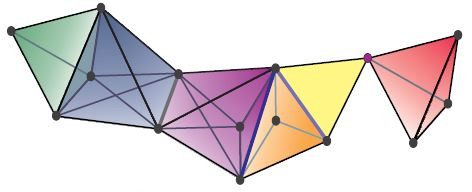
\includegraphics[width=0.75\textheight]{portada.jpg}}
\date{8 de noviembre de 2019}
\subject{Topología Algebraica}
\setbeamercolor{title}{fg=color}
\setbeamercolor{frametitle}{fg=color}
\setbeamercolor{structure}{fg=color}
\setbeamercovered{transparent}
\setbeamertemplate{navigation symbols}{}

\begin{frame}
\titlepage
\end{frame}

\begin{frame}{La categoría $\ordcat$ de ordinales finitos}
\begin{defs} La categoría $\ordcat$ de ordinales finitos \texttt{}tiene por objetos a los conjuntos $\nat{n} := \{0 < 1 < \dots < n\}$ y por flechas a los morfismos de posets $f : \nat{n} \to \nat{m}$.
\end{defs}

\begin{defs} Definimos para cada $n \in \N_0$ e $i \in \ord{n}$ los mapas de \textbf{cocaras} 
\begin{align*}
d^i : \ord{n-&1} \to \ord{n}\\
&j \mapsto \begin{cases}
j &\text{si $j < i$}\\
j+1 &\text{si $j \geq i$}
\end{cases}
\end{align*}
y los mapas de \textbf{codegeneraciones}
\begin{align*}
s^i : \ord{n+&1} \to \ord{n}\\
&j \mapsto \begin{cases}
j &\text{si $j \leq i$}\\
j-1 &\text{si $j > i$}
\end{cases}
\end{align*}
\end{defs}
\end{frame}

\begin{frame}{La categoría $\ordcat$ de ordinales finitos}
\begin{prop} Toda flecha $\ord{n} \xrightarrow{f} \ord{m}$ en $\ordcat$ se puede escribir como una composición de mapas de cocaras y codegeneraciones.
\end{prop}

\begin{prop} Los mapas de cocaras y codegeneraciones satisfacen las siguientes \textbf{identidades cosimpliciales},
\[
\begin{cases}
d^jd^i = d^id^{j-1} &\text{si $i < j$}\\
s^jd^i = d^is^{j-1} &\text{si $i < j$}\\
s^jd^j = s^jd^{j+1} = 1\\
s^jd^i = d^{i-1}s^j &\text{si $i > j+1$}\\
s^js^i = s^is^{j+1} &\text{si $i \leq j$}\\
\end{cases}
\]
\end{prop}
\end{frame}

\begin{frame}{Conjuntos Simpliciales}

\begin{defs} Un \textbf{conjunto simplicial} es un funtor $X : \ordcat^{op} \to \cat{Set}$. Concretamente, éste consiste de 
\begin{itemize}
\item[(i)] una sucesión de conjuntos $X_0,X_1,X_2, \dots$, y \item[(ii)] para cada $n \in \N_0$ e $i \in \ord{n}$, funciones 
$d_i : X_n \to X_{n-1}$ y $s_i : X_n \to X_{n+1}$ llamadas mapas de caras y degeneraciones respectivamente, que satisfacen las siguientes \textbf{identidades simpliciales}:
\[
\begin{cases}
d_id_j = d_{j-1}d_i &\text{si $i < j$}\\
d_is_j = s_{j-1}d_i &\text{si $i < j$}\\
d_js_j = d_{j+1}s_j = 1\\
d_is_j = s_jd_{i-1} &\text{si $i > j+1$}\\
s_is_j = s_{j+1}s_i &\text{si $i \leq j$}\\
\end{cases}
\] 
\end{itemize}
\end{defs}
\end{frame}

\begin{frame}{Conjuntos Simpliciales - Ejemplos}
\begin{center}
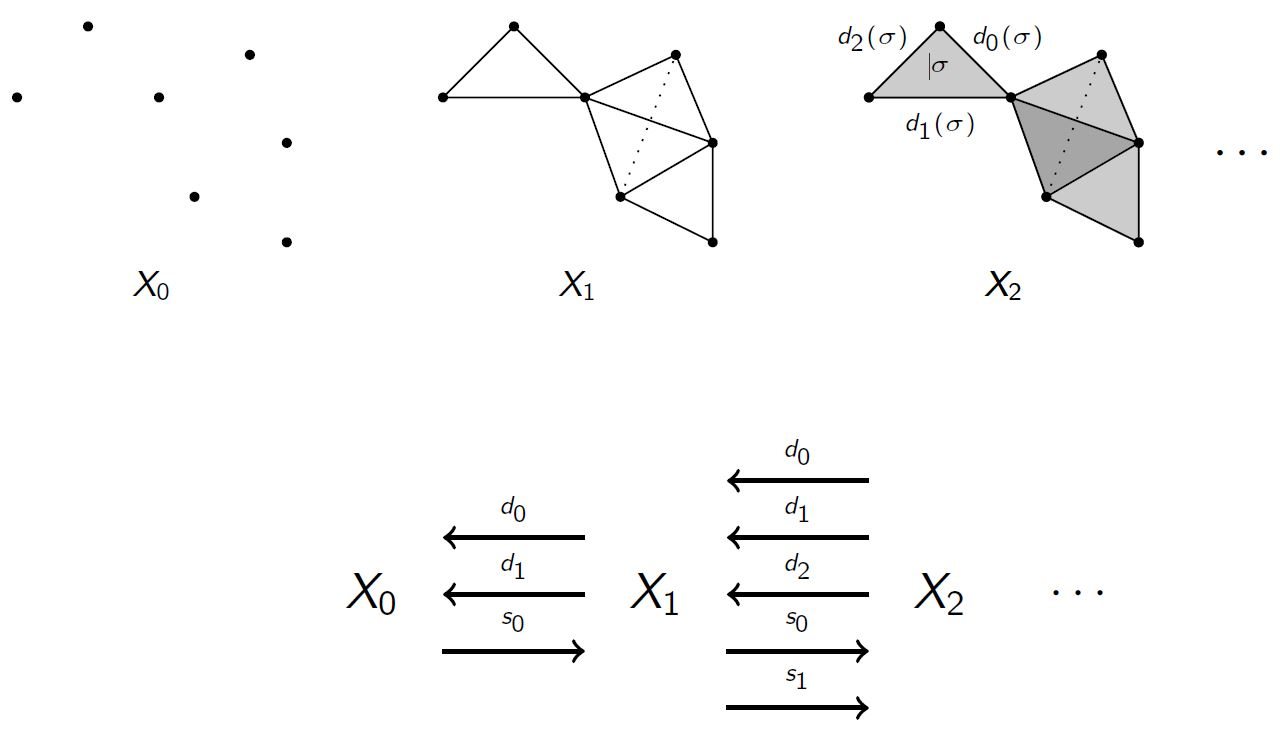
\includegraphics[width=0.75\textwidth]{SimplicialSetsIdea.jpg}
\end{center}
\begin{itemize}
\item <2-> Los complejos simpliciales ordenados
\item <3-> El espacio clasificante $BG$ de un grupo $G$
\item <4-> El nervio $N\mathscr{C}$ de una categoría $\mathscr{C}$
\item <5-> Los símplices singulares $\mathscr{S}(X)$ de un espacio topológico $X$
\end{itemize}
\end{frame}

\begin{frame}{Conjuntos Simpliciales  - Homología}
\begin{defs} Dado un conjunto simplicial $X$, definimos su \textbf{complejo de Moore} como el complejo de cadenas
\[
\cdots \to \Z X_2 \xrightarrow{\partial} \Z X_1 \xrightarrow{\partial} \Z X_0,
\]
con $\Z X_n$ el grupo abeliano libre generado por el conjunto $X_n$ y el borde
\[
\partial = \sum_{i=0}^n(-1)^i d_i
\]
para cada $n \geq 0$. La \textbf{homología} $H_\bullet(X)$ de $X$ es la homología de este complejo de cadenas.
\end{defs}
\begin{itemize}
\item <2-> $K \rightsquigarrow H_\bullet(K)$
\item <3-> $BG \rightsquigarrow H_\bullet(G)$
\item <4-> $\mathscr{S}(X) \rightsquigarrow H_\bullet(X)$
\end{itemize}
\end{frame}

\begin{frame}{Símplices Degenerados}
\begin{defs} Sea $X$ un conjunto simplicial. Un $n$-simplex $x \in X_n$ se dice \textbf{degenerado} si existe $y \in X_{n-1}$ tal que $s_i(y) = x$ para algún $i \in \ord{n}$. En caso contrario, decimos que $x$ es \textbf{no degenerado} y notamos 
\[
NX_n := \{x \in X_n : \text{ $x$ es no degenerado}\}.
\]
\end{defs}

\begin{prop}<2->  Sea $X$ un conjunto simplicial. Si $x \in X$ es un símplex degenerado, entonces existe un único símplex no degenerado $y \in X$ y mapas de degeneración $s_{i_1},\dots, s_{i_k}$ tales que $x = s_{i_1} \cdots s_{i_k}y$.
\end{prop}
\end{frame}

\begin{frame}{Morfismos Simpliciales}

\begin{defs} Dados dos complejos simpliciales $X,Y : \ordcat^{op} \to \cat{Set}$, un \textbf{morfismo de conjuntos simpliciales} de $X$ a $Y$ es una transformación natural $f : X \to Y$. Concretamente, esto consiste en dar una familia de funciones $f_n : X_n \to Y_n$ tales que para cada $0 \leq i \leq n$  los siguientes diagramas conmutan,
\begin{center}
\begin{tikzpicture}[ampersand replacement=\&, column sep=small]
\matrix (m) [matrix of math nodes,row sep=3em,column sep=4em,minimum width=2em]
  {
     X_n \& X_{n-1} \& \& X_n \& X_{n+1}\\
     Y_n \& Y_{n-1} \& \& Y_n \& Y_{n+1}\\};
  \path[-stealth]
    (m-1-1) edge node [left] {$f_n$} (m-2-1)
    (m-1-4) edge node [left] {$f_n$} (m-2-4)
    (m-1-2) edge node [right] {$f_{n-1}$} (m-2-2)
    (m-1-5) edge node [right] {$f_{n+1}$} (m-2-5)
    (m-1-1) edge node [above] {$d_i$} (m-1-2)
    (m-2-1) edge node [below] {$d_i$} (m-2-2)
    (m-1-4) edge node [above] {$s_i$} (m-1-5)
    (m-2-4) edge node [below] {$s_i$} (m-2-5);
\end{tikzpicture} 
\end{center}
\end{defs}
\end{frame}



\begin{frame}{Morfismos Simpliciales - Ejemplos}
\begin{itemize}
\item <1-> Un morfismo $f \colon (K,\leq) \to (L,\preceq)$ de complejos simpliciales ordenados induce un morfismo simplicial $f : K \to L$ entre los conjuntos simpliciales inducidos %via
%\[
%f_n([v_{i_0}, \dots, v_{i_n}]) = [f(v_{i_1}), \dots, f(v_{i_n})].
%\]
\item <2-> Un morfismo de grupos $\varphi : G \to H$ induce un morfismo simplicial $\varphi : BG \to BH$ entre sus espacios clasificantes %definido por
%\[
%\varphi_n(g_0, \dots,g_n) = (\varphi(g_0),\dots,\varphi(g_n)).
%\]
\item <3-> Un funtor $F : \mathscr{C} \to \mathscr{D}$ induce un morfismo simplicial $NF : N\mathscr{C} \to N\mathscr{D}$ entre los nervios
\item <4-> Una función continua $f : X \to Y$ entre dos espacios induce un morfismo simplicial $f_* : \mathscr{S}(X) \to \mathscr{S}(Y)$ entre sus complejos singulares
\end{itemize}
\begin{obs} <5-> Todas estas asignaciones son funtoriales. En particular, se tiene el \textbf{funtor singular} $\mathscr{S} : \cat{sSet} \to \cat{Top}$.
\end{obs}
\end{frame}

%\begin{frame}{Subcomplejos, Productos, Coproductos}
%
%\begin{defs} Sea $X$ un conjunto simplicial. Un \textbf{subconjunto simplicial} o subcomplejo %de $X$ es un conjunto simplicial $K$ que satisface $K_n \subseteq X_n$ para cada $n \geq 0$ y %cuyos mapas de caras y degeneraciones están dados por (co)restringir los de $X$.
%\end{defs}
%
%\begin{defs} Dados dos conjuntos simplciales $X$ e $Y$ se define su \textbf{producto} $X %\times Y$ como el conjunto simplicial dado por
%\[
%(X \times Y)_n := X_n \times Y_n, \quad d_i = d_i^X \times d_i^Y, \quad s_i = s_i^X \times %s_i^Y.
%\]
%para cada $0 \leq i \leq n$.

%De forma similar, su \textbf{coproducto} $X \sqcup Y$ es el conjunto simplicial dado por
%\[
%(X \sqcup Y)_n := X_n \sqcup Y_n, \quad d_i = d_i^X \sqcup d_i^Y, \quad s_i = s_i^X \sqcup %s_i^Y.
%\]
%para cada $0 \leq i \leq n$.
%\end{defs}
%\end{frame}
%
%\begin{frame}{Complejos de Funciones}
%\begin{defs} Sean $X$ e $Y$ conjuntos simpliciales. Definimos el \textbf{complejo de f %unciones} $\homcomplex(X,Y)$ dado por
%\[
%\homcomplex(X,Y)_n := \hom_{\cat{sSet}}(X \times \ss{n},Y)
%\]
%para cada $n \in \N_0$ y 
%\begin{align*}
%\theta^* : \homcomplex(X,&Y)_m \to \homcomplex(X,Y)_n \\
%&f \longmapsto f \circ (1_X \times \theta)
%\end{align*}
%para cada $\ord{n} \xrightarrow{\theta} \ord{m}$.
%\end{defs}
%\end{frame}
%
%\begin{frame}{Ley Exponencial}
%\begin{defs} Dados $X$ e $Y$ conjuntos simpliciales, se define la \textbf{función evaluación}
%\[
%ev : X \times \homcomplex(X,Y) \to Y.
%\]
%dada por $ev_n(x,f) = f(x,1_n)$. Esta resulta un morfismo simplicial que natural en ambas %variables.
%\end{defs}
%
%\begin{teo}[Ley Exponencial] Si $K,X$ e $Y$ son conjuntos simpliciales, la aplicación
%\begin{align*}
%ev_* : \hom_{\cat{sSet}}(K,\homcomplex(X,Y&)) \to \hom_{\cat{sSet}}(X \times K,Y)\\
%&g \longmapsto ev \circ (1_X \times g)
%\end{align*}
%está bien definida y es biyectiva. Más aún, esta resulta natural en las tres variables.\qed
%\end{teo}
%\end{frame}


\begin{frame}{Realización Geométrica}
\begin{defs} Sea $X$ un conjunto simplicial. Dotando a cada conjunto $X_n$ de la topología discreta, definimos la \textbf{realización geométrica} de $X$ como el espacio topológico 
\[
|X| := \left(\coprod_{n \geq 0}X_n \times |\ss{n}|\right)\Big/\sim
\]
donde identificamos a los puntos \[(x,|d^i|(p)) \sim (d_i(x),p)\] y \[(x,|s^i|(p)) \sim (s_i(x),p)\] para cada mapa de cocara y codegeneración.
\end{defs}
\end{frame}

\begin{frame}{Realización Geométrica - Ejemplos}
\begin{itemize}
\item <1-> La realización geométrica de $\ss{n}$ es homeomorfa al $n$-símplex topológico estándar.
\item <2-> En general, si $K$ es un complejo simplicial ordenado, la realización geométrica de su conjunto simplicial asociado es homeomorfa a la realización geométrica como complejo simplicial.
\item <3-> Una posible realización de la $n$-esfera: podemos dar un conjunto simplicial con sólo dos símplices no degenerados cuya realización geométrica sea homeomorfa a la esfera \guill{pegando los bordes de un $(n-1)$-símplex en un punto}.
\begin{center}
\begin{overprint}
\onslide <1>
\onslide <2>
\onslide <3>
\begin{center}
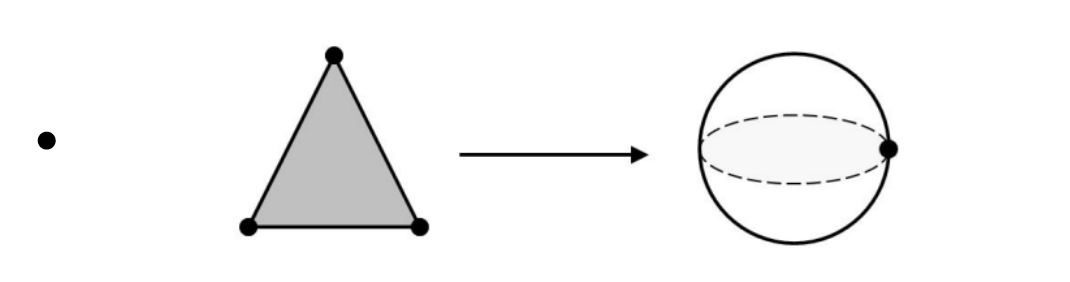
\includegraphics[width=0.75\textwidth]{modelo-simpl-nesfera.png}
\end{center}
\end{overprint}
\end{center}
\end{itemize}
\end{frame}

%\begin{frame}{Realización Geométrica - Puntos No Degenerados}
%\begin{defs} <1-> Sea $k \in \N_0$. Un punto $p \in |\ss{k}|$ del $k$-símplex topólogico se dice %\textbf{interior} si no existe un mapa de cocara $d^i : \ss{k-1} \to \ss{k}$ y $q \in |\ss{k-1}|$ %tal que $|d^i|(q) = p$.
%\end{defs}
%
%\begin{prop} <2-> Sea $k \in \N_0$ y $p \in |\ss{k}|$. Si $p$ es interior, existen únicos $l \in %\N_0$, $q \in |\ss{l}|$ y $d^{i_1}, \dots, d^{i_s}$ mapas de cocara tales que $p = |d^{i_1} \cdots %d^{i_s}|(q)$. En particular, si $p \in |\ss{k+1}|$ es interior, y $s^j$ es un mapa de %codegeneración, entonces $s_j(p)$ es interior. 
%\end{prop}
%
%\begin{defs} <3-> Sea $X$ un conjunto simplicial. Un punto $(x,p) \in \coprod_{n \geq 0} X_n %\times |\ss{n}|$ se dice \textbf{no degenerado} si $p$ es interior y $x$ no degenerado.
%\end{defs}
%
%\begin{lema} <4-> Sea $X$ un conjunto simplicial. Si $(x,p) \in \coprod_{n \geq 0} X_n \times %|\ss{n}|$, entonces existe un único punto no degerado $(y,q)$ relacionado con $(x,p)$.
%\end{lema}
%\end{frame}

\begin{frame}{Realización Geométrica - La adjunción $| \cdot | \dashv \mathscr{S}(-)$}
\begin{prop} <1-> Se tiene un funtor  $| \cdot | : \cat{sSet} \to \cat{Top}$ que asigna a cada conjunto simplicial $X$ su realización geométrica, y a cada morfismo simplicial $f : X \to Y$ una flecha $|f| : |X| \to |Y|$ inducida por la familia de funciones $\{f_n \times 1 : X_n \times |\ss{n}| \to Y_n \times |\ss{n}|\}_{n\geq 0}$.
\end{prop}


\begin{teo} <2-> Existe una adjunción
\begin{center}
\begin{tikzcd}[ampersand replacement=\&, column sep=small]
   \cat{sSet} \arrow[bend left=35]{rr}{| \  \cdot \ |}
  \& \rotatebox{90}{$\vdash$}
  \& \cat{Top} \arrow[bend left=35]{ll}{\mathscr{S}}
\end{tikzcd}
\end{center}
En otras palabras, se tiene una biyección $\cat{Top}(|X|,Y) \simeq \cat{sSet}(X,\mathscr{S}(Y))$ entre las funciones continuas $|X| \to Y$ y los morfismos simpliciales $X \to \mathscr{S}(Y)$. Más aún, esta biyección es natural tanto en $X$ como en $Y$.
\end{teo}
\end{frame}

\begin{frame}{Esqueletos}
\begin{defs} Sea $X$ un conjunto simplicial y $n \in \N_0$. Definimos el $n$-esqueleto $\sk_n X$ de $X$ como el menor subcomplejo de $X$ que tiene a los $j$-símplices de $X$ para cada $j \in \natzero{n}$. Es decir, es el complejo
\[
(\sk_nX)_j = \begin{cases}
X_j &\text{si $j \leq n$}\\
\{x \in X_j : x = s_{i_1} \cdots s_{i_{j-n}}y \text{ con } y \in X_n\} &\text{si $j > n$}
\end{cases}
\]
junto con las restricciones de los mapas de caras y degeneraciones de $X$. 

Se tienen además las siguientes inclusiones,
\end{defs}
\[
\sk_0X \subset \sk_1X \subset \sk_2X \subset \cdots \subset \sk_nX \subset \cdots
\]
\end{frame}

\begin{frame}{Esqueletos}
\begin{lema}<1-> Si $X$ es un conjunto simplicial, entonces $X \simeq \operatorname{colim_{n \geq 0}} \sk_nX$ donde el colímite se toma sobre el diagrama inducido por las inclusiones entre los $n$-esqueletos.
\end{lema}
\begin{lema}<2-> Si $X$ es un conjunto simplicial y $n \in \N$, entonces el siguiente diagrama
\begin{center}
\begin{tikzcd}[ampersand replacement=\&, column sep=small]
\coprod_{n \in NX_n} \partial \ss{n} \arrow[hook]{d}{}\arrow{r}\& \sk_{n-1}X\arrow[hook]{d}{}\\
\coprod_{n \in NX_n} \ss{n} \arrow{r}\& \sk_nX\\
\end{tikzcd}
\end{center}
es un puhsout.
\end{lema}
\end{frame}

\begin{frame}{Realización Geométrica - CW Aproximación}
\begin{obs} <1-> La realización geométrica $| \cdot | : \cat{sSet} \to \cat{Top}$ preserva colímites. En particular, preserva coproductos y pushouts.
\end{obs}

\begin{teo} <2-> La realización geométrica de un conjunto simplicial $X$ es un CW-complejo, con una celda por cada símplex no degenerado.
\end{teo}

\begin{teo} <3-> Si $X$ es un espacio topológico, la counidad de la adjunción $\eta_X : |\mathscr{S}(X)|\to X$ es una equivalencia débil. Concretamente, si $f : X \to Y$ es una función continua entonces el diagrama
\begin{center}
\begin{tikzcd}[ampersand replacement=\&, column sep=small]
\text{$|\mathscr{S}(X)|$} \arrow{r}{|Sf|}\arrow{d}{\eta_X} \& \text{$|\mathscr{S}(Y)|$} \arrow{d}{\eta_Y}\\
X \arrow{r}{f} \& Y
\end{tikzcd}
\end{center}
conmuta, y tanto $\eta_X$ como $\eta_Y$ son equivalencias débiles.
\end{teo}
\end{frame}


\begin{frame}{Categorías de modelos y categorías de homotopía}
\begin{itemize}
\item Podemos generalizar la noción de fibraciones, cofibraciones, y equivalencias débiles a otros contextos
\item <2-> Si $\mathscr{C}$ es una categoría de modelos, podemos considerar su categoría de homotopía $\cat{Ho}(\mathscr{C})$
\item <3-> 	La adjunción que vimos induce una adjunción
\begin{center}
\begin{tikzcd}[ampersand replacement=\&, column sep=small]
    \cat{Ho}(\cat{sSet}) \arrow[bend left=15]{rr}{| \  \cdot \ |_\ast}
  \& \rotatebox{90}{$\vdash$}
  \& \cat{Ho}(\cat{Top}) \arrow[bend left=15]{ll}{\mathcal{S}_\ast}
\end{tikzcd}
\end{center}
que es una equivalencia de categorías. Esto dice que \guill{las teorías de homotopía de espacios y conjuntos simpliciales son en esencia la misma}
\item <4-> ¿Qué es la teoría de homotopía simplicial?
\end{itemize}
\end{frame}

\begin{frame}{Fibraciones de Kan}
\begin{defs} <1-> Un morfismo simplicial $f : X \to Y$ se dice una \textbf{fibración de Kan} (o simplemente una fibración) si para cada diagrama conmutativo de la forma
\begin{center}
\begin{tikzcd}[ampersand replacement=\&, column sep=small]
\horn{n}{k} \arrow{r}\arrow[hook]{d} \&X\arrow{d}{f} \\
\ss{n} \arrow{r}\arrow[dashed]{ru}{\exists} \&Y
\end{tikzcd}
\end{center}
existe una flecha $\ss{n} \to X$ que sigue haciendo conmutar el diagrama.
\end{defs}
\end{frame}

\begin{frame}{Complejos de Kan}
\begin{defs} <1-> Un conjunto simplicial $X$ se dice un \textbf{complejo de Kan} si el morfismo simplicial $X \xrightarrow{!\exists} \ss{0}$ es una fibración de Kan.

Equivalentemente, 
\begin{itemize}
\item <2-> Un conjunto simplicial $X$ es un complejo de Kan sí y sólo si para cada morfismo simplicial $\alpha : \horn{n}{k} \to X$ tenemos una extensión $\overline{\alpha} : \ss{n} \to X$ al $n$-símplex,
\begin{center}
\begin{tikzcd}[ampersand replacement=\&, column sep=small]
\horn{n}{k} \arrow{r}{\alpha}\arrow[hook]{d} \& X \\
\ss{n} \arrow[dashed]{ru}[below]{\quad \exists \ \overline{\alpha}}
\end{tikzcd}
\end{center}
\item <3-> Un conjunto simplicial $X$ es un complejo de Kan sí y sólo si para cada $n$-upla de $(n-1)$-símplices $(x_0,\dots,\widehat{x}_k,\dots, x_n)$ de $X$ tales que $d_ix_j = d_{j-1}x_i$ si $i < j, \ i,j \neq k$, existe un $n$-símplex $x \in X_n$ tal que $d_ix = x_i$ para cada $i$.
\end{itemize}
\end{defs}
\end{frame}

\begin{frame}{Complejos de Kan}
\begin{prop} Una función continua $f : X \to Y$ es una fibración de Serre sí y sólo si el morfismo simplicial $\mathscr{S}(f) : \mathscr{S}(X) \to \mathscr{S}(Y)$ es una fibración de Kan.
\end{prop}
\begin{center}
\begin{tikzcd}[ampersand replacement=\&, column sep=small]
\text{$|\horn{n}{k}|$} \arrow{r}\arrow[hook]{d} \& X\arrow{d}{f} \\
\text{$|\ss{n}|$}\arrow[dashed]{ru}{\exists} \arrow{r} \&Y
\end{tikzcd}
\quad$\leftrightsquigarrow$\quad
\begin{tikzcd}[ampersand replacement=\&, column sep=small]
\text{$\horn{n}{k}$} \arrow{r}\arrow[hook]{d} \& \mathscr{S}(X)\arrow{d}{\mathscr{S}(f)} \\
\text{$\ss{n}$}\arrow[dashed]{ru}{\exists} \arrow{r} \&\mathscr{S}(Y)
\end{tikzcd}
\end{center}

\begin{prop} Si $X$ es un espacio topológico, entonces $\mathscr{S}(X)$ es un complejo de Kan. 
\end{prop}
\begin{center}
\begin{tikzcd}[ampersand replacement=\&, column sep=small]
\text{$|\horn{n}{k}|$} \arrow{r}{\alpha}\arrow[hook]{d} \& X \\
\text{$|\ss{n}|$} \arrow[dashed]{ru}[below]{\quad \exists \ \overline{\alpha}}
\end{tikzcd}
\quad$\leftrightsquigarrow$\quad
\begin{tikzcd}[ampersand replacement=\&, column sep=small]
\horn{n}{k} \arrow{r}{\alpha}\arrow[hook]{d} \& \mathscr{S}(X) \\
\ss{n} \arrow[dashed]{ru}[below]{\quad \exists \ \overline{\alpha}}
\end{tikzcd}
\end{center}
\end{frame}

\begin{frame}{Homotopía Simplicial}
\begin{columns}
\begin{column}{0.5\textwidth}
\vspace{5pt}

Una \textbf{homotopía} entre dos morfismos simpliciales $f,g : X \to Y$ es un morfismo simplicial $H : X \times \ss{1} \to Y$ que vale $f$ al restringir el $1$-símplex en una cara y $g$ al restringir a la otra.
\vspace{30pt}

Ésta se dice \textbf{relativa} a un subcomplejo $K$ de $X$ si además es \guill{constante en $K$}.
\end{column} 
\begin{column}{0.5\textwidth}  \begin{center}
\begin{tikzcd}[ampersand replacement=\&, column sep=small]
X \times \ss{0} \arrow{d}[left]{1 \times d_1}\arrow{r}{\simeq}\&X \arrow{d}{f}\\
X \times \ss{1} \arrow{r}{H}\&Y\\
X \times \ss{0} \arrow{u}{1 \times d_0}\arrow{r}{\simeq}\&X \arrow{u}[right]{g}
\end{tikzcd}
\end{center}
\begin{center}
\begin{tikzcd}[ampersand replacement=\&, column sep=small]
X \times \ss{1} \arrow{r}{H}\&Y\\
K \times \ss{1} \arrow[hook]{u}{i \times 1}\arrow{r}{\pi_1}\&K \arrow{u}[right]{\alpha}
\end{tikzcd}
\end{center}
\end{column}
\end{columns}
\end{frame}

\begin{frame}{Homotopía Simplicial}
\begin{prop} Si $X$ es un complejo de Kan, entonces las homotopías simpliciales de vértices definen una relación de equivalencia en $X_0$.
\end{prop}
\begin{obs} En particular esto nos dice que $\ss{1}$ \textbf{no} es un complejo de Kan.
\end{obs}
\begin{prop} Sea $X$ un conjunto simplicial e $Y$ un complejo de Kan. Si $K$ es un subcomplejo de $Y$, las homotopías simpliciales relativas a $K$ definen una relación de equivalencia en $\hom_{\cat{sSet}}(X,Y)$.
\end{prop}
\end{frame}

\begin{frame}{Grupos de Homotopía} 

\begin{defs} Sea $X$ un complejo de Kan y $n \in \N$. Se define el $n$-ésimo grupo de homotopía con punto base $v \in X_0$ como el conjunto $\pi_n(X,v)$ de clases de homotopía relativas a $\partial \ss{n}$ de morfismos simpliciales $\alpha : \ss{n} \to X$ que valen constantemente $v$ en el borde del símplex,
\begin{center}
\begin{tikzcd}[ampersand replacement=\&, column sep=small]
\ss{n} \arrow{r}{\alpha}\&X\\
\partial \ss{n} \arrow[hook]{u} \arrow{r}{\exists!} \&\ss{0}\arrow{u}{v}
\end{tikzcd}
\end{center}
\end{defs}
\begin{teo} Si $X$ es un complejo de Kan y $v \in X_0$ un vértice, entonces $\pi_n(X,v)$ es un grupo para todo $n \in \N$.
\end{teo}
\end{frame}

\begin{frame}{Modelos Minimales}

\begin{defs} <1-> Decimos que un complejo de Kan $M$ es un \textbf{complejo minimal} si cada vez que se tienen dos $n$-símplices $x,y \colon \ss{n} \to M$  homotópicos relativos a $\partial \ss{n}$ se tiene que $x = y$.
\end{defs}

\begin{lema} <2-> Sea $X$ un conjunto simplicial. Si $x,y \in X_n$ son dos símplices degenerados tales que $\partial x = \partial y$, entonces $x = y$. 
\end{lema}

\begin{prop} <3-> Si $X$ es un complejo de Kan, entonces existe un subcomplejo minimal $i : M \hookrightarrow X$ y una retracción $r : X \to M$ tal que $ir \simeq 1_X$. 
\end{prop}

\begin{teo} <4-> Sea $M$ un complejo minimal y $f : M \to M$ un morfismo simplicial. Si $f \simeq 1$, entonces $f$ es un isomorfismo. En particular, dos complejos minimales homotópicamente equivalentes son isomorfos.
\end{teo}
\end{frame}
\begin{frame}
\begin{center}
\scshape \LARGE ¡Fin!
\end{center}
\end{frame}

\end{document}